\documentclass{book}

\usepackage[utf8]{inputenc}  % para que funcionen las tildes
\usepackage{amsmath}
\usepackage{amssymb}
\usepackage{amsthm}
\usepackage{letltxmacro}
\LetLtxMacro\amsproof\proof
\LetLtxMacro\amsendproof\endproof
\usepackage{txfonts}
\usepackage{lmodern}
\usepackage[dvipsnames]{xcolor}
\usepackage{thmtools, thm-restate}
\usepackage{datetime} % para la hora de compilación
\usepackage{graphicx}
\graphicspath{{images/}}
\usepackage[spanish,es-noquoting]{babel} % es-noquoting es para que funcione tikz
\usepackage{mathabx} % para \divides
\usepackage{centernot} % para \centernot\inculdes
\usepackage{wrapfig}
\usepackage{multicol}
\usepackage{subcaption}
\usepackage{xfrac}
\usepackage{glossaries}
\usepackage{standalone}
\usepackage{pgfmath}
\usepackage{pgfplots}
\usepackage{pdfpages}
\usepackage{tikz}
\usetikzlibrary{arrows.meta}
\usetikzlibrary{shapes}
\usetikzlibrary{decorations.text}
\usetikzlibrary{positioning}
\usetikzlibrary{external}
\tikzexternalize[prefix=./tikzbuild/]
\tikzexternalize % activate!

\AtBeginDocument{%
  \LetLtxMacro\proof\amsproof
  \LetLtxMacro\endproof\amsendproof
}

\definecolor{coolblack}{rgb}{0.0, 0.18, 0.39}
%\usepackage[a6paper,margin=5mm]{geometry}
\usepackage[a4paper, top=2.5cm,bottom=2.5cm,left=2.5cm,right=2.5cm]{geometry}

%\setlength{\parindent}{0pt}
\usepackage{parskip}

\usepackage{hyperref}

% ESTILOS DE DEFINICIONES Y TEOREMAS
\declaretheoremstyle[
	bodyfont=\normalfont,
	shaded={
		margin=8pt,
		bgcolor=White,
		rulecolor=Black,
		rulewidth=1pt
}]{mythm}

\declaretheoremstyle[
	bodyfont=\normalfont,
	shaded={
		margin=1em,
		bgcolor={rgb}{0.9,0.9,0.9}
}]{mydfn}

\declaretheoremstyle[
bodyfont=\normalfont,
spacebelow=1em,
spaceabove=1em,
]{myej}

\declaretheoremstyle[
bodyfont=\normalfont,
spacebelow=1em,
spaceabove=1em,
shaded={
    margin=8pt,
    bgcolor=White,
    rulecolor=coolblack,
    rulewidth=1pt
}]{thej}

\declaretheoremstyle[
bodyfont=\normalfont,
spacebelow=1em,
spaceabove=1em,
thmbox=M
]{myeg}

% DEFINICIONES DE ENTORNOS DE TEOREMAS
\declaretheorem[
	name=Teorema,
	refname={teorema,teoremas},
	Refname={Teorema,Teoremas},
	style=mythm
]{thm}

\declaretheorem[
	name=Corolario,
	refname={corolario,corolarios},
	Refname={Corolario,Corolarios},
	style=myej
]{cor}

\declaretheorem[
	name=Proposici\'{o}n,
	refname={proposici\'{o}n,proposiciones},
	Refname={Proposici\'{o}n, Proposiciones},
	sharenumber=thm,
	style=myej
]{pro}

\declaretheorem[
name=Lema,
refname={lema,lemas},
Refname={Lema, Lemas},
sharenumber=thm,
style=myej
]{lm}

%\newtheorem*{cor}{Corolario}
\newtheorem*{lem}{Lema}

\declaretheorem[
	name=Definici\'{o}n,
	refname={definici\'{o}n,definiciones},
	Refname={Definici\'{o}n,Definiciones},
	style=mydfn
]{dfn}

\declaretheorem[
name=Ejercicio,
refname={ejercicio,ejercicios},
Refname={Ejercicio,Ejercicios},
style=myej,
numbered=no
]{ex}

\declaretheorem[
name=Ejercicio propuesto,
refname={ejercicio,ejercicios},
Refname={Ejercicio,Ejercicios},
style=thej,
]{th_ex}

\declaretheorem[
name=Ejemplo,
refname={ejemplo,ejemplos},
Refname={Ejemplo,Ejemplos},
style=myeg
]{eg}

\declaretheorem[
name=Observaci\'{o}n,
refname={observaci\'{o}n,observaciones},
Refname={Observaci\'{o}n,Observaciones},
style=myej,
numbered=no
]{obs}

\makeglossaries
\newglossaryentry{di}{name={DI},description={Dominio de integridad (ver \autoref{dfn:dominiointegridad})}}
\newglossaryentry{dip}{name={DIP},description={Dominio de ideales principales (ver \autoref{dfn:dominioidealesprincipales})}}
\newglossaryentry{dfu}{name={DFU},description={Dominio de factorización única (ver \autoref{dfn:dfu})}}
\newglossaryentry{de}{name={DE},description={Dominio euclídeo (ver \autoref{dfn:de})}}


\setcounter{chapter}{-1}
%COMANDOS ÚTILES PARA DERIVADAS
\AtBeginDocument{\renewcommand{\d}{\mathrm{d}}}
\newcommand{\Dd}[1]{\frac{\mathrm{d}}{\mathrm{d}#1}}
\newcommand{\dd}[2]{\frac{\mathrm{d}#1}{\mathrm{d}#2}}
\newcommand{\mbf}[1]{\mathbf{#1}}
% COMANDOS ÚTILES PARA LA TEORÍA DE GRUPOS
%\newcommand{\normsub}{\mathbin{\triangleleft}}
\newcommand{\normsub}{\lhd}
\newcommand{\uds}[1]{\mathcal{U}(#1)}
\newcommand{\inv}[1]{#1^{-1}}
\newcommand{\ima}{\text{Im }}
\newcommand{\isom}{\simeq}
\newcommand{\autom}[1]{\text{Aut}(#1)}
\newcommand{\gen}[1]{\langle#1\rangle}
\newcommand{\biy}[1]{\text{Biy}(#1)}

%\DeclareMathSymbol{\varprod}{\mathop}{largesymbolsA}{16}

\newcommand{\hr}{\rule{\textwidth}{.4pt}}
\newcommand{\N}{\mathbb{N}}
\newcommand{\Z}{\mathbb{Z}}
\newcommand{\R}{\mathbb{R}}
\newcommand{\Q}{\mathbb{Q}}
\newcommand{\C}{\mathbb{C}}
\renewcommand{\P}{\mathcal{P}}
\newcommand{\ZnZ}{\mathbb{Z}/n\mathbb{Z}}
\newcommand{\ZmZ}{\mathbb{Z}/m\mathbb{Z}}
\newcommand{\0}{\mathbf{0}}
\newcommand{\1}{\mathbf{1}}
\newcommand{\gr}{\text{gr }}


\renewcommand\qedsymbol{$\diamondsuit$}

\title{Apuntes de Ecuaciones Diferenciales}
\author{Rafael S\'{a}nchez S\'{a}nchez}
\begin{document}
\begin{titlepage}
	
\includepdf{portada.pdf}
\end{titlepage}


Revisión del \today $ $ a las \currenttime.

\begin{center}

\end{center}

\tableofcontents
% !TeX root = ../ecuaciones-diferenciales.tex

\chapter{Notación}
\begin{multicols}{2}
    \begin{itemize}
        \item $ \mathcal{P} \equiv f(x) = g(x)$, $\mathcal{P}$ es una ecuación.
        \item $\mbf{y} = f(x)$, $\mbf{y}$ es una variable dependiente.
        \item $\dd{y}{x} = y' = y_x$, derivada de y respecto de x.
    \end{itemize}
\end{multicols}

\part{Primer parcial}
% !TeX root = ../ecuaciones-diferenciales.tex

\chapter{Introducci\'{o}n a las ecuaciones diferenciales}

\section{Idea intuitiva}
\begin{dfn}[Ecuacion diferencial de primer orden]
	Sea $\mbf{y} = f(x)$, una \textbf{ecuación diferencial de primer orden} es una ecuación de la forma: $\mbf{y'}=F(x,\mathbf{y})$.\\
    Sea $g(x)$ una función de x, diremos que es solución cuando la ecuación diferencial se cumpla para $\mbf{y} = g(x)$.
\end{dfn}

Veamos unos ejemplos típicos.

\begin{eg}
    Consideramos $\P \equiv x'(t) = 2x(t)$ (o alternativamente $\mbf{x}' = 2\mbf{x}$)\\
    Vemos que es una ecuación diferencial de primer orden ya que sigue la definición anterior. Es sencillo ver que $F(t,\mbf{x}) = 2\mbf{x} = 2x(t)$. Queremos hallar que funciones resuelven $P$\\
    Además, observamos que si $x(t) = e^{2t}$, entonces $x'(t) = 2e^{2t} = 2x(t)$ y por tanto $x(t) = e^{2t}$ es una solución de $P$.\\Si pensamos con más cuidado también observamos que $x(t) = 7e^{2t}$ también satisface $P$.\\
    Nos interesaría entonces hallar una \textbf{solución general}, que con una sola ecuación englobe todas las soluciones. Aunque de momento no podemos justificarlo, si tomamos $x(t) = ae^{2t} \mid a \in \R$ entonces se cumple que $x'(t) = 2ae^{2t} = 2x(t)$ y por tanto es la solución general de $P$.
\end{eg}

Del ejemplo anterior surgen problemas llamados \textit{problema de valor inicial}, donde hallando la solución general y sabiendo la imagen de un punto $t_0$ por medio de $x(t)$ podemos determinar el parámetro y encontrar una solución explícitamente. Como continuación al ejemplo anterior consideremos el sistema:
$$
    \begin{cases}
        x'(t) = 2x(t) \\ x(0) = 8
    \end{cases}
$$
Para resolverlo, hallamos la solución general $x(t) = ae^{2t}$ y sustituimos la segunda ecuación. $x(0) = ae^{0} = 8 \implies a = 8$.

\begin{eg}
    Consideramos $\P \equiv x'(t) = 3(x(t))^{\sfrac{2}{3}}.$, queremos hallar \textit{la} solución para $x(0)=0$.\\
    Empezamos hallando soluciones a la ecuación, en este caso $x(t) = t^3$ y $x(t) = 0$ resuelven la ecuación. Nuestro sistema sería:
    $$
        \begin{cases}
            x'(t) = 3(x(t))^{\sfrac{2}{3}} \\ x(0) = 0
        \end{cases}
    $$
    Sin embargo, tanto $x(t) = t^3 \mid t = 0$ como $x(t) = 0$ resuelven $P$. No podemos hablar de \textit{la} solución puesto que hay dos.
\end{eg}

En los dos ejemplos anteriores tenemos una ecuación diferencial de la forma $\mbf{x'} = F(t, \mbf{x})$, $f(\mbf{x}) = 2\mbf{x}$ y $f(\mbf{x}) = 3\mbf{x}^{\sfrac{2}{3}}$ respectivamente. Sin embargo, en la segunda tenemos dos soluciones para $x(0) = 0$. Al observar las gráficas de las dos funciones se ve la razón a simple vista, la segunda no es derivable en $0$.
\begin{center}
    \begin{tikzpicture}
        \begin{axis}[domain=-5:5,samples=150,
        restrict y to domain=-10:10,
        xtick=\empty,ytick=\empty,
        %extra x ticks={0.8,1.4}, linea vertical
        %extra y ticks=3.333333,extra y tick labels={$\frac{10}{3}$}, linea horizontal
        grid=both,axis lines=middle
        ]
            \addplot+[no marks, thick] ({x},{2*x}) node[pos=0.3, below, sloped] {$f(x)=2x$};
            \addplot+[no marks, black, thick,samples=400] ({x},{3*x^(2/3)}) node[near end, below, sloped] {$f(x)=3x^{\sfrac{2}{3}}$};
            \addplot+[no marks, black, thick,samples=400] ({-x},{3*x^(2/3)});
        \end{axis}
    \end{tikzpicture}
\end{center}

\begin{eg}[Crecimiento de una población]
    Consideramos $\P \equiv \mbf{x'} = \lambda \mbf{x}$. ($\lambda$ típicamente es natalidad o mortalidad).\\
    Sabiendo que modela el crecimiento de una población en función del tiempo, podemos aproximar (veremos por qué más adelante)
    $\frac{\Delta x}{\Delta t} \sim \dd{x}{t} = \mbf{x'}$. Por tanto (como $\lamda$ es una tasa, se entiende que el tiempo tiende a 0 para hallarla):
    $$ \frac{\Delta x}{\Delta t}\sim \dd{x}{t} = \lambda \cdot \mbf{x} \implies \lambda = \lim_{t \to 0} \frac{\mbf{x'}}{\mbf{x}}$$.
\end{eg}

El crecimiento de una población de organismos lo suficientemente grandes no se ve representada por la ecuación anterior debido a la limitación de recursos. Interesaría por tanto modelizar la ecuación teniendo esto en cuenta. Para ello utilizaremos el parámetro $L$ como el límite al que tendería la población con los recursos existentes.

\begin{eg}[Crecimiento de una población con limitación de recursos]
    Consideramos $\P \equiv \mbf{x'} = a(1-\frac{\mbf{x}}{L})\mbf{x}$ con $a > 0$. De esta forma cuando $\mbf{x} << L$ o $\mbf{x} >> L$ , tenemos prácticamente la ecuación del ejemplo anterior. Si $\mbf{x} \sim L$ entonces la población apenas crece/decrece. Para encontrar soluciones a esta ecuación no hace falta resoverla, basta graficarla. Partimos de $\mbf{x'} = f(t, \mbf{x}) = a (1 - \frac{\mbf{x}}{L})\mbf{x}$.
    \\
    \begin{center}
        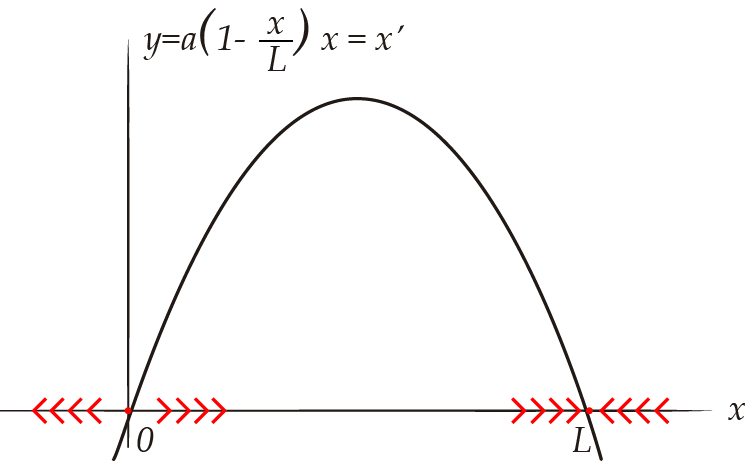
\includegraphics{1-limiterecursos.png}\label{img:1-limiterecursos}
    \end{center}
    Es fácil ver que $\mbf{x'}$ es una parábola, que corta al eje X en $0$ y $L$. Además, se indica con (>>) la dirección en la que se mueve $x(t)$ conforme avanza $t$. Tanto $0$ como $L$ son puntos de equilibrio, repulsor (inestable) y atractor (estable) respectivamente.
\end{eg}
\break

\begin{wrapfigure}{r}{0.5\textwidth}
  \begin{center}
    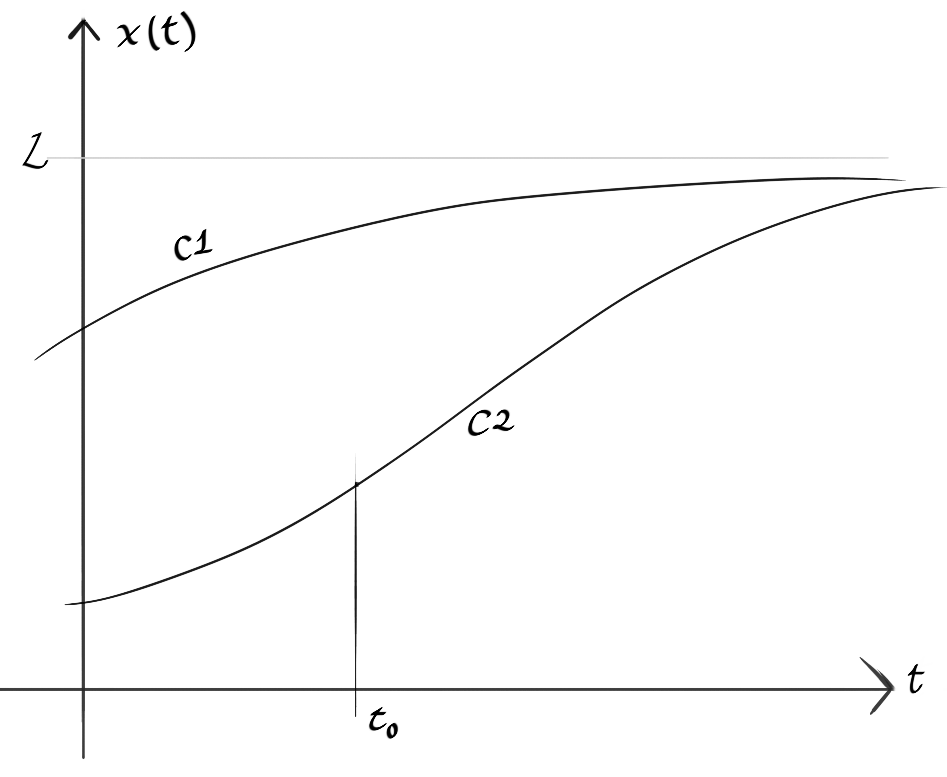
\includegraphics[width=0.48\textwidth]{1-poblaciontiempo.png}
  \end{center}
  \caption{Población - Tiempo}\label{img:1-poblaciontiempo}
\end{wrapfigure}
Habiendo encontrado las soluciones de la funcion anterior, nos preguntamos como varía la población frente al tiempo. Más adelante veremos formalmente como representar $\mbf{x}$ frente a $t$. Sin embargo, podemos razonar el aspecto de la función.
Sabemos que tiene que corregirse cerca de L, y que si $\mbf{x} << L$ entonces tiene un crecimiento parecido al exponencial. Por tanto, podría tener el aspecto de la figura \ref{img:1-poblaciontiempo}.
De este gráfico podemos deducir varias cosas. Para empezar, sabemos que $\mbf{x''}(t_0)=0$ tiene solución para la curva $c_2$ ya que tiene un punto de inflexión. Además, observamos disintos tipos de crecimiento en función del valor de $x(0)$ por lo que tendría sentido intentar determinar para qué valores $x_0$ obtenemos el crecimiento de $c_1$ y para cuáles el de $c_2$.

\begin{th_ex}\label{thex:29/01-0}
    ¿Para qué valores de $x_0$ se dan los diferentes crecimientos de $c_1$ y $c_2$?.\\
    \textit{Sugerencia}: Considerar el problema de valor inicial con $x''(t_0) = 0$.
\end{th_ex}

\section{Método de separación de variables}
Esta sección trata sobre el primer método de resolución de ecuaciones diferenciales. Antes de definir el método formalmente vamos a ver un ejemplo.
\begin{eg}[Resolución sencilla]
    Sea $\P \equiv \mbf{y'} = x\mbf{y}$. Halla las soluciones de la ecuación.\\
    $\mbf{y'} = \dd{y}{x}$, con esta igualdad podemos hacer manipulaciones sin justificar (de momento).
    $$
        \dd{y}{x} = x \mbf{y} \implies \frac{dy}{\mbf{y}} = x\mathrm{d}x \implies \int \frac{dy}{\mbf{y}} = \int x\mathrm{d}x \implies \log|\mbf{y}| = \frac{x^2}{2} + C \implies |\mbf{y}| = e^{\sfrac{x^2}{2} + C} = e^C \cdot e^{\sfrac{x^2}{2}}
    $$
    $$
        \mbf{y} = \pm e^C \cdot e^{\sfrac{x^2}{2}} = ke^{\sfrac{x^2}{2}} \mid k \in \R
    $$
\end{eg}
Esta resolución se conoce como método de separación de variables.
\begin{th_ex}\label{thex:29/01-1}
    Resolver $\P \equiv \mbf{x'} = a(1-\sfrac{\mbf{x}}{L})\mbf{x}$ con $x(0)=0$.\\
\end{th_ex}
Vamos a generalizar el método por medio de la siguiente proposición.
\begin{pro}[Método de separación de variables]
    Sea $F(x)$ una primitiva de $f(x)$ y $G(\mbf{y})$ una primitiva de $g(\mbf{y})$, es decir, $\dd{F}{x} = f(x)$ y $\dd{G}{\mbf{y}} = g(\mbf{y})$, con $\mbf{y} = f(x)$. Y sea una ecuación $\P \equiv \dd{y}{x} = \frac{f(x)}{g(\mbf{y})}$, entonces las soluciones de $\P$ cumplen:
    $$
        G(y(x)) = F(x) + \mathcal{C} \mid \mathcal{C}\ constante.
    $$
\end{pro}

\begin{proof}
    \begin{align*}
        \intertext{Por la regla de la cadena:}
            &\Dd{x} G(y(x)) = \dd{G}{\mbf{y}}(y(x)) \cdot \dd{y}{x}(x) \\
        \intertext{Como $\dd{G}{\mbf{y}} = g(\mbf{y})$ y $\dd{y}{x} = \frac{f(x)}{g(\mbf{y})}$   por hipóstesis:}
            &\dd{G}{\mbf{y}}(y(x)) \cdot \dd{y}{x}(x) = g(y(x)) \cdot \frac{f(x)}{g(y(x))} = f(x) = \Dd{x} F(x)
        \intertext{Es decir:}
            &\Dd{x}G(y(x)) = \Dd{x}F(x) \implies \Dd{x}G(y(x)) - \Dd{x}F(x) = 0 \implies G(y(x)) - F(x)  =  \mathcal{C} \implies G(y(x)) = F(x) + \mathcal{C}
    \end{align*}
\end{proof}
\begin{obs}
    La prosposición anterior está incompleta, faltaría ver que condiciones tienen que cumplir $f(x)$ y $g(\mbf{y})$. Para completarla tenemos que considerar la existencia de primitivas y la condición de que $\mathcal{C}$ sea constante.
    \begin{itemize}
        \item Ya que tenemos que usar que $F(x)$ y $G(\mbf{y})$ son primitivas, basta pedir que tanto $f(x)$ y $g(\mbf{y})$ sean continuas. Esto garantiza que $F(x)$ y $G(\mbf{y})$ son ambas $C^1$
        \item Si $h'(x) = 0 \implies h(x)$ constante en cada intervalo en que está definida (pues $\R$ es conexo). Si $h:\R \rightarrow \R$ entonces $h(x)$ es constante. Como $\mathcal{C}$ surge de integrar $0$ a la derecha de la ecuación, podemos afirmar que $\mathcal{C} = h(x)$ y por tanto constante.
    \end{itemize}
\end{obs}
\section{Significado geométrico de la ecuación diferencial ordinaria}
Vamos a analizar una ecuación diferencial de forma gráfica para interpretarla geométricamente. Consideramos $\mbf{y'} = f(x, \mbf(y))$. Supongamos que $\mbf{y}$ tiene la gráfica de la figura \ref{img:1-siggeom}.
\begin{figure}[h]
\begin{subfigure}{.5\textwidth}
    \centering
    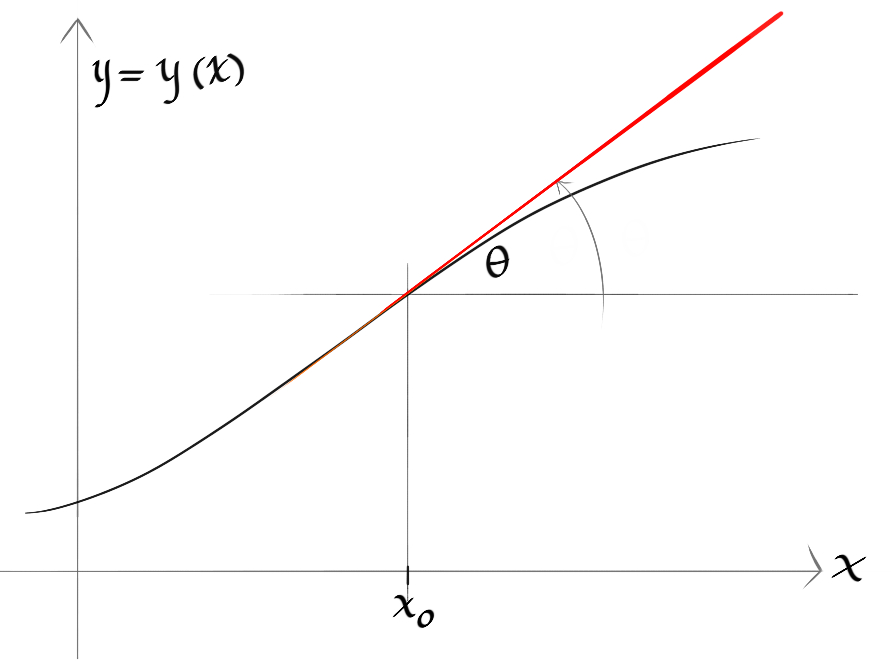
\includegraphics[width=1\textwidth]{1-significadogeom.png}
    \caption{Recta tangente en $x_0$ conocidas $\mbf{y}$ y $x_0$}\label{img:1-siggeom}
\end{subfigure}
\begin{subfigure}{.5\textwidth}
    \centering
    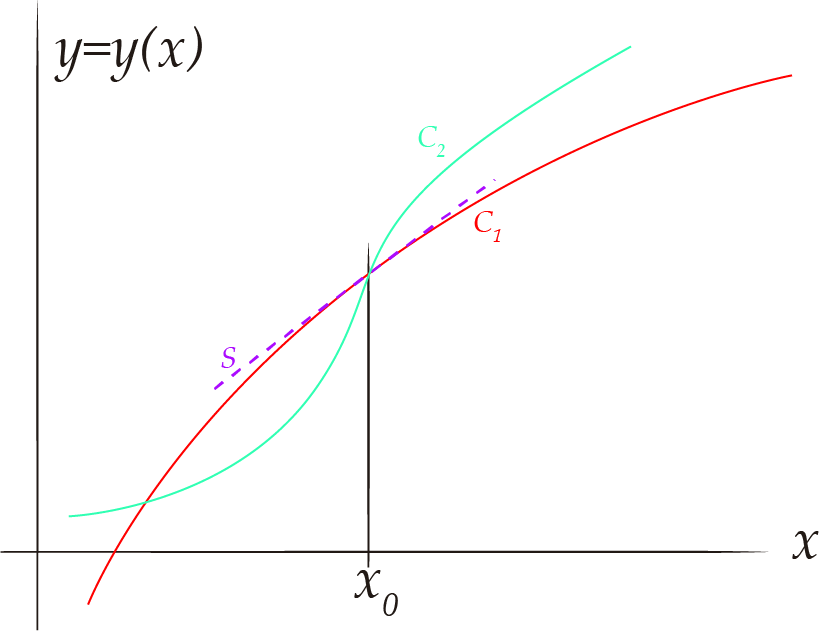
\includegraphics[width=1\textwidth]{1-significadogeom2.png}
    \caption{Curvas dadas el segmento $\mathcal{S}$.}\label{img:1-siggeom2}
\end{subfigure}
\end{figure}
Entonces, $\mbf{y'}(x_0) = \tan{\theta}$, que es la pendiente de la recta tangente a la gráfica de $\mbf{y}$ en $x_0$. Esto es cálculo elemental, lo que nos interesa es saber algo de la función $\mbf{y}$ cuando sabemos algo de $\mbf{y'}$.\\

Ilustramos en la figura \ref{img:1-siggeom2} entonces la casuística de conocer $\P \equiv \mbf{y'} = f(x,\mbf{y})$. En este caso, nos preguntamos que aspecto podría tener $\mbf{y}$ para que fuera solución de $\P$. Como conocemos $y'(x_0)$, podemos considerar que $\mathcal{S}$ es un semento paralelo a la recta tangente de la gráfica en $x_0$. Es fácil ver que $\mathcal{C}_1$ no puede ser solución de $\P$ pues $\mathcal{C}'_1(x_0) \neq y'(x_0)$. Sin embargo, es evidente que $\mathcal{C}_2$ sí resuelve $\P$.\\\\
Si repetimos el procedimiento de determinar como son las pendientes (como acabamos de hacer para $x_0$) para todos los puntos, hallamos el \textit{campo de pendientes}.

\begin{eg}[Hallar un campo de pendientes]
    Sea $\P \equiv \mbf{x'} = t^2 + \mbf{x}^2$, es decir, $f(t, \mbf{x}) = t^2 + \mbf{x}^2$. Si queremos hallar qué pendiente se le asigna al punto $p = (\sfrac{1}{\sqrt{2}},\sfrac{1}{\sqrt{2}})$ evaluamos la función $f$, $f(p) = 1$. Por tanto, la función $\mbf{x}$ que soluciona $\P$ tiene tangente con pendiente $1$ en $t = \sfrac{1}{\sqrt{2}}$.\\\\
    De hecho, es lógico pensar que a cualquier punto que cumpla $t^2 + \mbf{x}^2 = 1$ se le asignará una pendiente de $1$ a su recta tangente. Este conjunto de puntos conforman la \textbf{isoclina} de pendiente 1.\\\\
    De forma general, para una constante $c$ dada (en este ejemplo necesariamente no negativa pues $f(t, \mbf{x})$ es suma de cuadrados), podemos definir la isoclina de pendiente c:
    $$
    ISO_c = \left\{(t, \mbf{x}) \mid f(t, \mbf{x}) = c\right\}
    $$
    Volviendo a nuestro ejemplo, las isoclinas van a ser curvas que cumplan $t^2 + \mbf{x}^2 = c$ para un $c$ dado.\\
    \begin{minipage}[c]{0.3\linewidth}
      \begin{center}
          \raisebox{\dimexpr \topskip-\height}{
        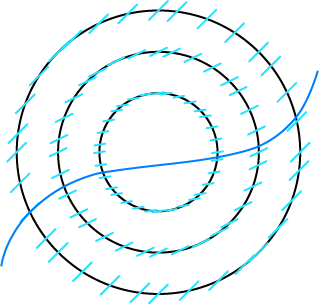
\includegraphics[width=\textwidth]{1-isoclinas.png}}
      \end{center}
    \end{minipage}\hfill
    \begin{minipage}[c]{0.65\textwidth}
        Hemos representado las isoclinas junto con un pequeño segmento de pendiente $c$ para disintos valores de $c$. Como las isoclinas cumplen que $t^2 + \mbf{x}^2 = c$, estas son las circumferencias de radio $\sqrt{c}$ con $c > 0$.\\
        Podemos observar tambien que $ISO_0 = \{(0,0)\}$ e $ISO_{c < 0} = \varnothing$.\\\\ Llamamos a la gráfica con pequeños segmentos \textit{campo de pendientes} y por tanto, una función que resuelva $\P$ tiene que ser tangente al segmento del punto por el que pase.
    \end{minipage}
    Sin embargo, los campos de pendientes permiten ver cómo es la función a grandes rasgos. En nuestro ejemplo parece indicar que $x(t) \uparrow \infty$, pero no sabemos si lo hace de forma asintótica ($x(t) \uparrow \infty$ en t finito), o x(t) crece a infinito cuando $t \rightarrow \infty$.\\
    Esto no puede resolverse gráficamente y veremos como resolverlo de forma analítica más adelante.
\end{eg}

\section{Ecuaciones diferenciales y problemas geométricos}
Gracias a la relación de la derivada con la tangencia de funciones, podemos plantear problemas geométricos en forma de ecuación diferencial.
\subsection{Trayectorias ortogonales}
De la recta tagente a un punto surge el concepto de recta normal a ese punto, que no es más que la recta perpendicular a la tangente y que pasa por dicho punto. Para ver como se relacionan estas dos rectas vamos a hacer un análisis simple. Diremos que dos curvas son ortogonales si en el punto de cruce las rectas tangentes a cada curva son perpendiculares entre sí.
\begin{wrapfigure}[20]{l}{0.5\textwidth}
  \begin{center}
    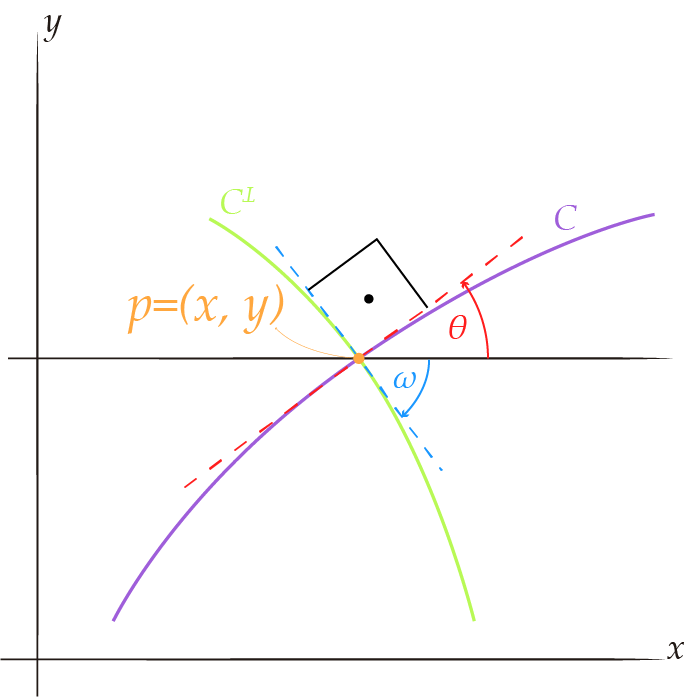
\includegraphics[width=0.48\textwidth]{1-trayectoriasortogonales.png}
  \end{center}
  \caption{Relaciones entre curvas ortogonales}\label{img:1-trayort}
\end{wrapfigure}
De la figura \ref{img:1-trayort} vemos que la pendiente de $C$ es $pend_C = \tan(\theta)$. Asimismo, $pend_{C^{\perp}} = \tan(\omega)$ y $\omega = \theta - \sfrac{\pi}{2}$. A partir de aquí desarrollamos:
$$
    \tan(\omega)=\frac{\sin(\theta-\sfrac{\pi}{2})}{\cos(\theta-\sfrac{\pi}{2})} = \frac{-\cos(\theta)}{\sin(\theta)} = -\frac{1}{\tan(\theta)}
$$
y por tanto,
\begin{equation} \label{eq:pendientes}
    pend_C \cdot pend_{C^{\perp}} = -1
\end{equation}

Nuestro objetivo es que dada una familia de curvas $fam_{C}$, podamos encontrar una (\textit{familia de}) curva que sea ortogonal a todas las de la familia en los puntos de cruce.\\\\
Supongamos que la familia original satisface una ecuación diferencial ordinaria $\mbf{y_1'} = f(x, \mbf{y_1})$. Queremos encontrar otra ecuación que defina a la ortogonal.\\\\
Como $fam_{C}$ sigue una EDO (\textit{ecuacion diferencial ordinaria}), podemos afirmar que $pend_{C} = \mbf{y_1'} = f(x, \mbf{y_1})$. Usando \ref{eq:pendientes}, $pend_{C^\perp} = \frac{-1}{f(x, \mbf{y_1})}$. Pero además, si $C^\perp$ sigue una EDO, está dada por una función $\mbf{y_2} = y_2(x)$ y entonces $\mbf{y_2'} = \frac{-1}{f(x, \mbf{y_1})}$.\\
Concluimos con que dada $fam_C$ descrita por $\mbf{y'}=f(x,\mbf{y})$, podemos encontrar $fam_{C^\perp}$ que satisface:
$$
    \mbf{y'} = -\frac{1}{f(x, \mbf{y})}
$$
\begin{eg}[Familia ortogonal a otra dada]
    Consideramos la familia: $x^2-\mbf{y}^2 = c \mid c \neq 0$\\
    Para cada $c$, eso define $\mbf{y}$ implícitamente en función de $x$.
    \begin{center}
        \vspace{1mm}
        \hfill
        \begin{tikzpicture}
            \begin{axis}[domain=-5:5,samples=150,
            restrict y to domain=-5:5,
            xtick=\empty,ytick=\empty,
            %extra x ticks={0.8,1.4}, linea vertical
            %extra y ticks=3.333333,extra y tick labels={$\frac{10}{3}$}, linea horizontal
            grid=both,axis lines=middle, axis equal
            ]
                \addplot+[no marks, thick, red, solid] ({x},{x}) node[pos=0.1, below, sloped] {$c=0$};
                \addplot+[no marks, thick, red, solid] ({x},{-x});
                %%%%%%%%%%%%%%%%%%%%%%%%%%%%%%%%%%%%%%%%%%%%%%%%%%%%%%%%%%%%%%%%%%%
                \addplot+[no marks, thick, coolblack, solid] ({(x^2+1)^(1/2)},{x}) node[pos=0.5, right] {$c > 0$};
                \addplot+[no marks, thick, coolblack, solid] ({-(x^2+1)^(1/2)},{x});
                \addplot+[no marks, thick, coolblack, densely dashed] ({(x^2+4)^(1/2)},{x});
                \addplot+[no marks, thick, coolblack, densely dashed] ({-(x^2+4)^(1/2)},{x});
                \addplot+[no marks, thick, coolblack, densely dotted] ({(x^2+9)^(1/2)},{x});
                \addplot+[no marks, thick, coolblack, densely dotted] ({-(x^2+9)^(1/2)},{x});
                %%%%%%%%%%%%%%%%%%%%%%%%%%%%%%%%%%%%%%%%%%%%%%%%%%%%%%%%%%%%%%%%%%%
                \addplot+[no marks, thick, black, solid] {(x^2+1)^(1/2)} node[pos=0.5, above, sloped] {$c < 0$};
                \addplot+[no marks, thick, black, solid] {-(x^2+1)^(1/2)};
                \addplot+[no marks, thick, black, densely dashed] {(x^2+4)^(1/2)};
                \addplot+[no marks, thick, black, densely dashed] {-(x^2+4)^(1/2)};
                \addplot+[no marks, thick, black, densely dotted] {(x^2+9)^(1/2)};
                \addplot+[no marks, thick, black, densely dotted] {-(x^2+9)^(1/2)};
            \end{axis}
        \end{tikzpicture}\hfill \break
        \vspace{1pt}
        $x^2-y^2=c$ para distintos valores de $c$.\\
        (También puede verse como las curvas de nivel del paraboloide hiperbólico)
    \end{center}
    \vspace{5pt}
    Para hallar la familia de curvas ortogonales vamos a seguir una serie de pasos:
    \begin{enumerate}
        \item \texttt{Encontrar una EDO que cumplan esas curvas.}\\
            $$
                x^2-\mbf{y}^2 = c \rightarrow \Dd{x} (x^2-y^2=c) \rightarrow 2x - 2\mbf{y}\mbf{y'} = 0 \implies \mbf{y'} = \frac{x}{\mbf{y}} = f(x,\mbf{y})
            $$
        \item \texttt{Econtrar la EDO para trayectorias ortogonales.}\\
            $$
                \mbf{y'} = -\frac{1}{f(x, \mbf{y})} = -\frac{\mbf{y}}{x}
            $$
        \item \texttt{Resolver la ecuación anterior}\\
            $$
                \dd{y}{x} = -\frac{\mbf{y}}{x} \implies -\frac{\mathrm{d}y}{\mbf{y}} = \frac{\mathrm{d}x}{x} \implies \log|y| = \log|x| + \mathcal{C}
            $$
            es decir,
            $$
                |\mbf{y}| = \frac{e^\mathcal{C}}{|x|} \implies |x\mbf{y}| = e^\mathcal{C} \implies x\mbf{y} = k : k = e^\mathcal{C} \lor k = e^{-\mathcal{C}} \implies \mbf{y} = \frac{k}{x}
            $$
    \end{enumerate}
    Con la solución general podemos representar parte de la familia:
    \begin{center}
        \vspace{1mm}
        \hfill
        \begin{tikzpicture}
            \begin{axis}[domain=-5:5,samples=150,
            restrict y to domain=-5:5,
            xtick=\empty,ytick=\empty,
            %extra x ticks={0.8,1.4}, linea vertical
            %extra y ticks=3.333333,extra y tick labels={$\frac{10}{3}$}, linea horizontal
            grid=both,axis lines=middle, axis equal
            ]
                \addplot+[no marks, very thin, black, solid] ({(x^2+1)^(1/2)},{x});
                \addplot+[no marks, very thin, black, solid] ({-(x^2+1)^(1/2)},{x});
                \addplot+[no marks, very thin, black, solid] ({(x^2+4)^(1/2)},{x});
                \addplot+[no marks, very thin, black, solid] ({-(x^2+4)^(1/2)},{x});
                \addplot+[no marks, very thin, black, solid] ({(x^2+9)^(1/2)},{x});
                \addplot+[no marks, very thin, black, solid] ({-(x^2+9)^(1/2)},{x});
                %%%%%%%%%%%%%%%%%%%%%%%%%%%%%%%%%%%%%%%%%%%%%%%%%%%%%%%%%%%%%%%%%%%
                \addplot+[no marks, thick, blue, solid, samples=500] {1/x};
                \addplot+[no marks, thick, blue, solid, samples=500] {-1/x};
                \addplot+[no marks, thick, blue, solid, samples=300] {4/x};
                \addplot+[no marks, thick, blue, solid, samples=300] {-4/x};
                \addplot+[no marks, thick, blue, solid] {9/x};
                \addplot+[no marks, thick, blue, solid] {-9/x};
            \end{axis}
        \end{tikzpicture}\hfill \break
        \vspace{1pt}
        En azul posibles soluciones para disintos valores de $k$, en negro la familia original\\
        Se observa que son curvas ortogonales a la familia original.
    \end{center}
\end{eg}


\part{Segundo parcial}

\part{Tercer parcial}

\part{Apéndices}

%\renewcommand{\chaptername}{Apéndice}
%\renewcommand{\thechapter}{\Alph{chapter}}
%\setcounter{chapter}{0}

%% !TeX root = ../apuntes-ea.tex

\chapter{Ejercicios}

\section{Hoja 1}

\begin{ex}[H1.2]
	Sean $a,b,c \in G = (-1,1)$. Probamos las propiedades de los grupos.
	\begin{itemize}
		\item \textbf{Asociatividad:}
		\begin{align*}
			(a \ast b) \ast c = \left(\frac{a+b}{1+ab}\right) \ast c = \frac{\left(\frac{a+b}{1+ab}\right) + c}{1 + \left(\frac{a+b}{1+ab}\right)c} = \frac{\frac{a+b+c+abc}{1+ab}}{\frac{1+ab+ac+bc}{1+ab}} = \frac{a+b+c+abc}{1+ab+ac+bc} \\
			a \ast (b \ast c) = a \ast \left(\frac{b+c}{1+bc}\right) = \frac{a+\left(\frac{b+c}{1+bc}\right)}{1+a\left(\frac{b+c}{1+bc}\right)} = \frac{\frac{a + b + c + abc}{1+bc}}{\frac{1+ab+ac+bc}{1+bc}} = \frac{a+b+c+abc}{1+ab+ac+bc}
		\end{align*}
		\item \textbf{Elemento neutro:} es el $0$ ya que $x\ast 0 = \frac{x+0}{1+x\cdot 0} = \frac{x}{1} = x$ y además $0 \ast x = \frac{0+x}{1+0\cdot x} = \frac{x}{1} = x$
		\item \textbf{Elemento inverso:} la ecuación
		\begin{align*}
			x \ast \inv{x} = 0 \iff \frac{x + \inv{x}}{1+x\inv{x}} = 0 \iff \inv{x} = -x
		\end{align*}
		siempre tiene solución y ocurre lo mismo para la ecuación $\inv{x} \ast x = 0 \iff \inv{x} = -x$
		\item \textbf{Clausura:} tenemos que probar que si $x,y \in (-1,1)$ entonces $x \ast y \in (-1,1)$. Consideramos $f(x,y) = x \ast y = \frac{x+y}{1+xy}$. Derivando tenemos que $\nabla f(x,y) = (\frac{1}{(1+xy)^2},\ \frac{1}{(1+xy)^2}) \neq 0, \forall x,y \in [-1,1]\times[-1,1]$. Si el máximo no se alcanza en ningún sitio de dentro del cuadrado $(-1,1)\times(-1,1)$ se tendrá que alcanzar en el borde.
		\begin{itemize}
			\item Fijado $x = 1$ tenemos que $f(1,y) = \frac{1+y}{1+y} = 1 \implies f(1, -1 < y < 1) < 1$ porque si $f(1, -1 < y < 1)$ tomara un valor mayor que $1$ habría un máximo en $(-1,1)\times(-1,1)$ y esto no puede ser pues $\nabla f$ no se anula en el cuadrado.
			\item Fijado $x = -1$ tenemos que $f(-1, y) = \frac{y-1}{1-y} = -1 \implies f(-1, -1 < y < 1) > -1$ por la misma razón que antes.
			\item Hacemos lo mismo fijando la $y$ y variando la $x$.
		\end{itemize}
		En el borde (que no está incluido) se alcanzan máximo y mínimo que acotan a $f$ en el cuadrado:
		\begin{align*}
			-1 < f(x,y) = x \ast y < 1,\quad \forall x, y \in G
		\end{align*}
	\end{itemize}
\end{ex}

\begin{ex}[H1.3]Hallar los inversos de los siguientes elementos, cada uno en su grupo correspondiente:
	\begin{enumerate}
		\item $o(\overline{11})$ en $\uds{\Z^\ast/23\Z}$ es $22$ porque $23 \cdot 22 \equiv 1 \mod 23$
		\item $o(\overline{5})$ en $\uds{\Z^\ast/31\Z}$ es $3$ porque $5 \cdot 3 \equiv 1 \mod 31$
	\end{enumerate}
\end{ex}

\begin{ex}[H1.33]
	\label{ex:h1.33}
	Sea $G$ un grupo. Suponed que existe un único $a \in G$ de orden 2. Demostrad que $a \in Z(G)$.
\end{ex}

\begin{proof}
	Recordamos que $a \in Z(G) \iff ga = ag,\ \forall g \in G$. Definimos el isomorfismo de conjugación $\phi_g (x) = gx\inv{g}$ para algún $g$. Como $\phi_g$ es isomorfismo lleva elementos de orden $n$ en elementos de orden $n$. Entonces $\phi_g(a) = a$ ya que $a$ es el único elemento de orden 2. Por tanto $ga\inv{g} = a \implies ga = ag \implies a \in Z(G)$.
\end{proof}

\section{Hoja 2}

\begin{ex}[H2.1]
	\label{ex:h2.1}
	Se considera el tercer grupo diédrico $D_3$. Se pide hallar lo siguiente:
	\begin{enumerate}
		\item Las clases de conjugación de cada uno de sus elementos.
		\begin{proof}
			Las clases dan una partición del grupo. Si un elemento pertenece a una clase, entonces la clase de ese elemento también es la clase a la que pertenece.
			\begin{itemize}
				\item $cl(e) = \{e\}$
				\item $cl(B)$? Sabemos que $|cl(B)| = [G:C(B)]$. Sabemos que $\gen{B} =\{1, B, B^2\} \subset C(B)$ luego $|C(B)| \geq 3$. Si hubiera más elementos en $C(B)$ tendríamos que $|C(B)| = 6$ pues $C(B) < D_3$. Esto no ocurre porque sabemos que $B$ no conmuta con todos los demás elementos. Por ejemplo $BA \neq AB$. Por tanto $|C(B)| = 3 \implies |cl(B)| = [D_3:C(B)]= 6/3 = 2$. Es claro que $B \in cl(B)$. Además, como $cl(B)$ contiene elementos transformados por el isomorfismo conjugación sabemos que el otro elemento que hay tiene orden 3. El único elemento que queda de orden 3 es $B^2 \implies cl(B) = \{B, B^2\}$.
				
				\item $cl(A)?$ Sabemos que $A$ no conmuta con todos ($A \not\in Z(D_3)$) luego $|C(A)| < 6$. Sabemos que $\gen{A} = \{1, A\} < C(A)$. Además, como $C(A)$ es un (sub)grupo sabemos que no puede haber más elementos porque si los hubiera, $|\gen{A}| \divides |C(A)| \implies C(A) \geq 6$ pero ya hemos visto que no puede ser. Es decir que $|cl(A)| = [D_3:D(A)] = 6 / 2 = 3$. Por tanto $cl(A)$ incluye los 3 elementos que nos quedan: $cl(A) = \{A, AB, AB^2\}$.
			\end{itemize}
		\end{proof}
	
		\item Los elementos de $\text{Int}(D_3)$.
		\item Los centralizadores $C_{D_3}(x)$ para cada $x \in D_3$
		\item Los normalizadores $N(H)$ para cada $H < D_3$.
	\end{enumerate}
\end{ex}

\begin{ex}[H2.2]
	
	\begin{proof}
		Obtenidas las clases en el ejercicio \nameref{ex:h2.1} se verifica que $|D_3| = |cl(e)| + |cl(B)| + |cl(A)| = 1 + 2 + 3 = 6$
	\end{proof}
	
\end{ex}

\begin{ex}[H2.6]
	Sea $G$ un grupo. ¿Verdadero o falso?
	\begin{enumerate}
		\item $H < G$ y $H$ conmutativo implica $H \normsub G$.
		\item $H < G$ y $|H| = 2$ implica $H \normsub G$.
		\item Si $\varphi: G \to G_1$ es un homomorfismo de grupos, entonces $\ima \varphi \normsub G$
		\item Si $H \normsub K$ y $K \normsub G$ entonces $H \normsub G$
		\item Si $H \normsub G$ y $|H| = m$ entonces $H$ es el único subgrupo de $G$ de orden $m$.
		\item Si $H \normsub G$ entonces $H < Z(G)$.
		\begin{proof}[FALSO]
			Contraejemplo: En $G = D_4$ tomamos $H = \gen{B^2} = \{1, B, B^2, B^3\} \not\subset Z(D_4) = \{1, B^2\}$.
		\end{proof}
	\end{enumerate}
\end{ex}

\begin{ex}[H2.10]
	\begin{proof}
		Fijado $n$ y definida $\alpha_n : G \to G,\ x \mapsto x^n$ tenemos que $\alpha_n$ es un homomorfismo de grupos. Además podemos expresar $H_2 = \ker \alpha_n \implies H_2 \normsub G$. Además también tenemos que $H_1 = \ima \alpha_n < G$. Veamos que $H_1 \normsub G$. Es decir, que $gH_1\inv{g} = H_1,\ \forall g \in G$. Para ello tomamos $x_1^n \in H_1$ y lo conjugamos $gx_1^n\inv{g} = (gx_1\inv{g})^n$ por ser $\alpha$ homomorfismo de grupos. En particular $(gx_1\inv{g})^n \in \ima \alpha \implies (gx_1\inv{g})^n \in H_1 \implies (gx_1\inv{g})^n = x_2^n$ para algún $x_2 \in H_1 \implies H_1 \normsub G$.
	\end{proof}
\end{ex}

\begin{ex}[H2.13] Si $A$ es un grupo abeliano con $n$ elementos y $k$ es un entero primo con $n$, demostrad que la aplicación $\varphi : A \to A$ definida por $\varphi(a) = a^k$ es un isomorfismo.
	\begin{itemize}
		\item $\varphi$ homomorfismo de grupos.
		\begin{proof}
			\begin{align*}
				\varphi(a)\varphi(b) = a^kb^k = (ab)^k = \varphi(ab)
			\end{align*}
		\end{proof}
		\item $\varphi$ biyectiva $\iff \varphi$ inyectiva ya que dominio y codominio coinciden
		\begin{proof}
			$\ker \varphi = \{a \in A \mid \varphi(a) = a^k = 1\}$. Probaremos que $a^k = 1 \iff a = 1$ y por tanto que $\ker \varphi = \{1\} \implies \varphi$ inyectiva. Sabemos que $a^k = 1 \iff o(a^k) = 1$. Sea $t = o(a) \divides n$. Distinguimos dos casos
			\begin{itemize}
				\item Si $t = 1$ entonces $a = 1$ y ya está
				\item Si $t > 1$ entonces $o(a^k) = \frac{t}{mcd(k, t)} = \frac{t}{1} > 1$ contradicción. Luego necesariamente $t = o(a) = 1$.
			\end{itemize}
		\end{proof}
	\end{itemize}
\end{ex}

\begin{ex}[H2.22]
	\label{ex:h2.22}
	Demostrad que si $G$ es un grupo no conmutativo y tiene orden $p^3$ ($p$ un número primo) entonces $Z(G)$ tiene orden $p$.
	
	\begin{proof}
		Sabemos que $Z(G) < G \implies |Z(G)| \divides |G| \implies |Z(G)| \in \{1, p, p^2, p^3\}$
		\begin{itemize}
			\item $|Z(G)| \neq p^3$ porque en tal caso $G$ sería conmutativo
			\item $|Z(G)| \neq 1$ porque $G$ es un p-grupo y por tanto su centro no es el trivial.
			\item Si $|Z(G)| = p^2$ entonces $|G/Z(G)| = p \implies G/Z(G)$ es cíclico lo que no es posible si $G$ no es abeliano.
		\end{itemize}
	
		Por descarte concluimos que $|Z(G)| = p$.
	\end{proof}
\end{ex}


\begin{ex}[H2.25]
	Sabemos que $\autom{\Z/12\Z} \isom \uds{\Z^\star/12\Z}$ donde $\Z^\star/12\Z$ es el grupo multiplicativo $(\{\overline{1}, \overline{2}, \overline{3}, \dots,  \overline{11}\}, \cdot)$. Queda $\uds{\Z^\star/12\Z} = (\{\overline{1}, \overline{5}, \overline{7}, \overline{11}\}, \cdot )$ y además da la casualidad que $\forall x \in \uds{\Z^\star/12\Z},\ o(x) = 2$ (todos los elementos son su propio inverso) por lo que no tenemos restricciones al definir $f: \Z/2\Z \to \autom{\Z/12\Z}$:
	\begin{align*}
		f:\Z/2\Z & \to \autom{\Z/12\Z} \isom \uds{\Z^\star/12\Z} \\
		e = \overline{0} &\mapsto 1 \\
		\overline{1} &\mapsto \{\overline{1}, \overline{5}, \overline{7}, \overline{11}\}
	\end{align*}
\end{ex}

\begin{ex}[H2.26]
	Sea $|G_1| = m, |G_2| = n,\ mcd(m, n) = 1$. Si $f:G_1 \to G_2$ es h. de g. sabemos que $o(f(a)) \divides o(a),\ \forall a \in G_1$. Además $o(a) \divides m \land o(f(a)) \divides n$ por el teorema de Lagrange (\ref{thm:lagrange}).
	\begin{align*}
		\begin{cases}
		o(a) \divides m \land o(f(a)) \divides n \\
		mcd(m, n) = 1 \\
		o(f(a)) \divides o(a)
		\end{cases} \implies o(a) = o(f(a)) = 1, \forall a \in G_1
	\end{align*}
	Por lo que solo puede haber un homomorfismo entre ellos y además es el trivial $f(a) = e_{G_2}$.
\end{ex}

\begin{ex}[H2.19]
	Definimos una función $f:[0, 2\pi] \subset \R \to \mathbb{S}^1, \alpha\mapsto \cos \alpha + i \sin \alpha$. Esta función tiene la propiedad de que $f(\alpha) \cdot f(\alpha') = \cos(\alpha + \alpha') + i\sin(\alpha + \alpha') = f(\alpha + \alpha')$ y por tanto es un h. de g.\footnote{A la izquierda (en $\R$) sumamos pero a la derecha (en $\mathbb{S}^1$) multiplicamos.} entre $R$ y $\mathbb{S}^1$.
	
	Un elemento de $\cos \alpha + i \sin \alpha \in \mathbb{S}^1$ es de torsión $\iff \exists n \mid (\cos \alpha + i \sin \alpha )^n = 1$. Ahora bien $(\cos \alpha + i \sin \alpha )^n = \cos n\alpha + i \sin n\alpha = 1 \iff n\alpha = k 2\pi$. 
\end{ex}

\section{Hoja 4}

\begin{ex}[H4.11] Hallar los subgrupos de Sylow de $S_5$.
	Sabemos que $|S_5| = 5! = 2^3\cdot3\cdot 5$ y por \nameref{thm:sylow1} tenemos lo siguiente:
	\begin{itemize}
		\item $\exists P_2,\ |P_2| = 2^3 = 8$.
		\item $\exists P_3,\ |P_3| = 3$. Además en $S_5$ hay $\binom{5}{3}2! =20 $ 3-ciclos y en cada $gP_3\inv{g} = \{1, a, a^2 \mid o(a) = 3\}$ hay 2 elementos de orden 3 distintos. Además, $g_1P_3\inv{g_1} \cap g_2P_3\inv{g_2} = \{e\}$ porque si su intersección fuera más grande entonces serían el mismo subgrupo (porque son cíclicos). Es por esto que tenemos que repartir 40 elementos dando 2 a cada 3-grupo con lo que obtenemos $n_3 = 20 / 2 = 10$ 3-subgrupos de Sylow en $S_5$.
		\item $\exists P_5,\ |P_5| = 5$. Además en $S_5$ hay $4! = 24$ 5-ciclos (elementos de orden 5) y en cada $gP_5\inv{g} = \{1, a, a^2, a^3, a^4 \mid o(a) = 5\}$ tenemos $4$ elementos de orden $5$ distintos. Además, $g_1P_5\inv{g_1} \cap g_2P_5\inv{g_2} = \{e\}$ porque si su intersección fuera más grande entonces serían el mismo. Así, tenemos $24$ 5-ciclos a repartir entre los diferentes $gP_5\inv{g}$ dando 4 5-ciclos a cada 1. Por tanto tenemos $n_5 = 24/4 = 6$ 5-subgrupos de Sylow en $S_5$.
	\end{itemize}
\end{ex}

\begin{ex}[H4.18]
	Demostrar que todo grupo de orden $|G| = 5^3 \cdot 7^3$ tiene un subgrupo normal de orden 125.
	
	\begin{proof}
		\nameref{thm:sylow1} $\implies \exists P_5 < G,\ |P_5| = 125$. \nameref{thm:sylow3} $\implies n_5 \divides 7^3 \land n_5 \equiv 1 \mod 5$ es decir $n_5 \in \{1, 7, 49, 343\} \land n_5 \in \{1, 6, 11, \dots\}$. Como ni $49$ ni $343$ son conguentes con $1$ módulo 5 tenemos que $n_5 = 1 \implies P_5 \normsub G$.
	\end{proof}
\end{ex}

\begin{ex}[H4.20] Hallad todos los grupos abelianos de órdenes 36, 64, 96 y 100.
	\begin{enumerate}
		\item $|G| = 36 = 2^2\cdot3^2$
		\begin{proof}
			\nameref{thm:sylow1} $\implies \exists P_2,\ |P_2| = 4 \land \exists P_3,\ |P_3| = 9$. Además $G$ abeliano $\implies P_2, P_3 \normsub G \implies G \isom P_2 \times P_3$. Estudiamos los grupos de orden 4 y de orden 9
			\begin{itemize}
				\item $|P_2| = 4$ entonces $P_2 \isom \Z/2\Z \times \Z/2\Z \lor P_2 \isom \Z/4\Z$
				\item $|P_3| = 9$ entonces $P_3 \isom \Z/3\Z \times \Z/3\Z \lor P_3 \isom \Z/9\Z$
			\end{itemize}
			Como $G \isom P_2 \times P_3$ tenemos 4 posibles grupos abelianos de orden 36.
		\end{proof}
	\end{enumerate}
\end{ex}

\begin{ex}[H4.22]
	Hallar todos los grupos abelianos de orden 175.
	
	\begin{proof}
		$|G| = 5^2\cdot 7$. Por el \nameref{thm:sylow1} tenemos que $\exists P_5, P_7 < G$ con $|P_5| = 25,\ |P_7| = 7$ y además por ser $G$ abeliano tenemos que $P_5, P_7 \normsub G \implies G \isom P_5 \times P_7$. Estudiamos los grupos de orden 25 y de orden 7:
		\begin{itemize}
			\item $|P_5| = 25 \land P_5$ abeliano $\implies P_5 \isom \Z/25\Z \lor P_5 \isom \Z/5\Z \times \Z/5\Z$. En ambos casos $P_5$ es producto directo de cíclicos pues $\Z/n\Z$ es cíclico.
			\item $|P_7| = 7 \land P_7$ abeliano $\implies P_7 \isom \Z/7\Z$. Ocurre lo mismo que con $P_5$.
		\end{itemize}
		Concluimos que $G \isom \Z/25\Z \times \Z/7\Z \lor G \isom \Z/5\Z \times \Z/5\Z \times \Z/7\Z$. Los dos casos son abelianos por ser producto directo de grupos cíclicos.
	\end{proof}
\end{ex}

\begin{ex}[H4.23]
	¿Cuántos elementos de orden 3 puede tener un grupo abeliano de orden 36?
	
	\begin{proof}
		$|G| = 36 = 2^2 3^2$. \nameref{thm:sylow1} $\implies \exists P_2, P_3 < G,\ |P_2| = 4,\ |P_3| = 9$. Estudiamos los grupos de órdenes 4 y 9:
		\begin{itemize}
			\item $|P_3| = 9 \implies P_3 \isom \Z/9\Z \lor P_3 \isom \Z/3\Z \times \Z/3\Z$
			% TODO: terminar
		\end{itemize}
	\end{proof}
\end{ex}

\chapter{Índices}

%%TODO por qué no podemos utilizar only= para hacer whitelisting en lugar de blacklisting? que alguien lo arregle parfavar
\renewcommand{\listtheoremname}{Lista de definiciones}
\listoftheorems[ignore={thm,ej,pro,cor,obs,lm,ex}]

\renewcommand{\listtheoremname}{Lista de teoremas}
\listoftheorems[onlynamed,ignore={dfn,ej,pro,cor,obs,lm,ex}]

\renewcommand{\listtheoremname}{Lista de ejemplos}
\listoftheorems[onlynamed,ignore={dfn,thm,pro,cor,obs,lm,ex}]

\renewcommand{\listtheoremname}{Lista de ejercicios}
\listoftheorems[onlynamed,ignore={dfn,thm,pro,cor,obs,lm,ej}]

\printglossaries

\bibliographystyle{alpha}
\bibliography{apuntes-ea}


\end{document}
